\documentclass[twoside,11pt]{article}

% JAGI template (template/jagi.sty, agi.bst, AGIS-logo-BW.png). Packages after jagi, as the template asks.
\usepackage{jagi}
\usepackage{times}
\usepackage{url}
\usepackage{booktabs}
\usepackage{tabularx}
\usepackage{array}
\usepackage{xcolor}
\usepackage{tikz}
\usetikzlibrary{positioning,arrows.meta,calc}
\usepackage{pgfplots}
\pgfplotsset{compat=1.16}

\newcolumntype{L}{>{\raggedright\arraybackslash}X}
\newcommand{\inr}{INR}

% Heading arguments: {volume}{issue}{pages}{year}{submitted}{accepted}{DOI}{short authors}.
% Not a journal submission: volume, pages, acceptance date and DOI are left as dashes.
\jagiheading{--}{--}{--}{2026}{2026-10-23}{--}{--}{Team AgentReel}
\ShortHeadings{AgentReel: A Grounded Multi-Agent Video Pipeline}{Team AgentReel}
\firstpageno{1}

\begin{document}

\title{AgentReel: A Grounded, Self-Checking Multi-Agent Pipeline\\for Institutional Awareness Videos on Two T4 GPUs}

% Team member names and e-mail addresses to be filled in.
\author{\name Author One \email author-one-email \\
       \name Author Two \email author-two-email \\
       \addr K J Somaiya School of Engineering, Somaiya Vidyavihar University\\
       Vidyavihar, Mumbai 400077, India}

\editor{}

\maketitle

\begin{abstract}
AgentReel turns a one-page brief card into a finished 30--60\,s awareness video for K J Somaiya in a single command. It runs nine LangGraph agents on one Kaggle notebook with two NVIDIA T4 GPUs, using only open-weight models and no paid API. Because no fact sheet was provided, a researcher agent discovers, saves and indexes official Somaiya and Indian-government pages at run time. Every claim must carry a verbatim quote that code finds in a saved source and that a natural-language-inference model accepts. A critic runs 51--59 deterministic and model-based checks and routes each failure back to the agent that owns it, for at most three repair loops, before a human reviews safety and responsible-AI topics. We describe the architecture and report the first end-to-end run on the brief C01 (``College AI policy explainer''): 65\,min, 208 logged calls, \inr~0, zero human interventions, and a spec-compliant 40\,s video that the reviewer approved. Re-reading that run's artifacts exposed three defects the critic did not catch. Images and the voice-over were reused across repair loops after the script and storyboard changed, so the final video narrated an earlier script than the one the critic checked. The contact whitelist also absorbed 88 URLs from one government report's bibliography. We report all three with their fixes, and argue that every check must be bound to the exact artifact it certifies.
\end{abstract}

\begin{keywords}
  multi-agent systems, retrieval-augmented generation, automated video generation, LLM critics, reproducibility, responsible AI
\end{keywords}

\section{Introduction}

The LY Agentic AI Laboratory evaluation at K J Somaiya School of Engineering asks two-person teams to build an agent pipeline that turns a sealed brief into a promotional or awareness video for the campus \citep{kjsce2026handout}. It is modelled on the AGEWEC 2026 challenge \citep{agewec2026}. A brief card names a topic, audience, format, duration, tone, items that must be included or avoided, and a call-to-action. Topics range from anti-ragging and mental-health support to admissions, responsible use of AI, festivals and the institution's research. On the day of the Live Run a team draws an unseen brief and has three hours to deliver. The run may use at most \inr~500 of paid APIs and at most five logged human interventions. Facts may come only from official sources, and the video must meet a fixed delivery specification.

Three properties of this setting shape the design. First, the topic is unknown until the run starts, so nothing in the pipeline may be topic-specific except the evidence it gathers. Second, no fact sheet or media kit was supplied, so the system must find its own official evidence and prove that every on-screen claim and contact comes from it; a fabricated fact costs ten marks and a wrong helpline zeroes the accuracy score. Third, the whole system must run on free hardware with open models and be reproducible from one command, with a tamper-evident log of every call.

This paper makes four contributions:
\begin{itemize}
\item A nine-agent LangGraph pipeline \citep{langgraph2026} that runs end to end on two T4 GPUs with open-weight models (Section~\ref{sec:system}).
\item A grounding procedure in which claims survive only if a quoted span is found verbatim in a saved official source and accepted by an NLI model, and contacts are extracted from source text by pattern, never generated (Section~\ref{sec:grounding}).
\item A critic that routes each failed check to the agent that owns it, with a regression guard and a policy for soft findings (Section~\ref{sec:critic}).
\item A case study of the first real run, including three defects found by auditing its artifacts after the fact, and the general lesson they teach (Sections~\ref{sec:case} and \ref{sec:findings}).
\end{itemize}

\section{System Overview}
\label{sec:system}

The only input is a brief file, \path{briefs/<ID>.yaml}, typed from the card. One command runs everything:
\begin{verbatim}
    python run.py --brief briefs/C01.yaml --seed 42
\end{verbatim}
Figure~\ref{fig:graph} shows the agent graph. The graph runs top to bottom; images are generated per shot in parallel with the voice-over. When a hard check fails, the critic writes feedback for the most upstream agent responsible and the graph re-runs from that agent, taking earlier stages from a cache. Categories A (safety) and C (responsible AI) always stop for human review, as the handout requires; the review is logged as a checkpoint, not as an intervention.

\begin{figure}[t]
\centering
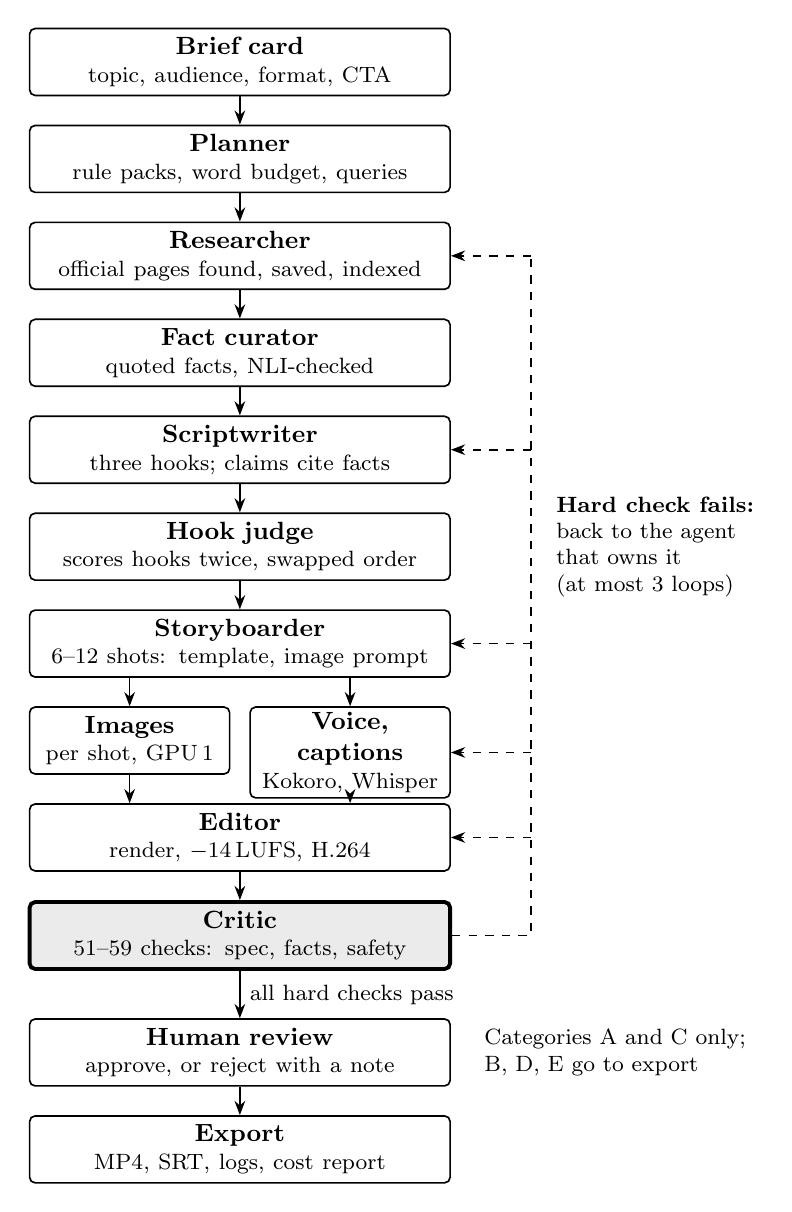
\begin{tikzpicture}[
  node distance=3.6mm,
  box/.style={draw, rounded corners=2pt, align=center, text width=52mm, minimum height=8.5mm,
              font=\small, line width=0.6pt, inner sep=2pt},
  half/.style={box, text width=24mm},
  arr/.style={-{Stealth[length=1.8mm]}, line width=0.6pt},
  back/.style={-{Stealth[length=1.8mm]}, dashed, line width=0.6pt},
]
\node[box] (brief) {\textbf{Brief card}\\[-1pt]\footnotesize topic, audience, format, CTA};
\node[box, below=of brief] (planner) {\textbf{Planner}\\[-1pt]\footnotesize rule packs, word budget, queries};
\node[box, below=of planner] (research) {\textbf{Researcher}\\[-1pt]\footnotesize official pages found, saved, indexed};
\node[box, below=of research] (curator) {\textbf{Fact curator}\\[-1pt]\footnotesize quoted facts, NLI-checked};
\node[box, below=of curator] (script) {\textbf{Scriptwriter}\\[-1pt]\footnotesize three hooks; claims cite facts};
\node[box, below=of script] (hook) {\textbf{Hook judge}\\[-1pt]\footnotesize scores hooks twice, swapped order};
\node[box, below=of hook] (story) {\textbf{Storyboarder}\\[-1pt]\footnotesize 6--12 shots: template, image prompt};
\node[half, below=3.6mm of story.south west, anchor=north west] (img) {\textbf{Images}\\[-1pt]\footnotesize per shot, GPU\,1};
\node[half, below=3.6mm of story.south east, anchor=north east] (voice) {\textbf{Voice, captions}\\[-1pt]\footnotesize Kokoro, Whisper};
\node[box, below=3.6mm of img.south west, anchor=north west] (editor) {\textbf{Editor}\\[-1pt]\footnotesize render, $-14$\,LUFS, H.264};
\node[box, below=of editor, line width=1.4pt, fill=black!8] (critic) {\textbf{Critic}\\[-1pt]\footnotesize 51--59 checks: spec, facts, safety};
\node[box, below=6mm of critic] (review) {\textbf{Human review}\\[-1pt]\footnotesize approve, or reject with a note};
\node[box, below=of review] (export) {\textbf{Export}\\[-1pt]\footnotesize MP4, SRT, logs, cost report};

\foreach \a/\b in {brief/planner, planner/research, research/curator, curator/script, script/hook,
                   hook/story, editor/critic, review/export}
  \draw[arr] (\a) -- (\b);
\draw[arr] (img.north |- story.south) -- (img.north);
\draw[arr] (voice.north |- story.south) -- (voice.north);
\draw[arr] (img.south) -- (img.south |- editor.north);
\draw[arr] (voice.south) -- (voice.south |- editor.north);
\draw[arr] (critic) -- node[right, font=\footnotesize] {all hard checks pass} (review);

\coordinate (rail) at ($(critic.east)+(10mm,0)$);
\draw[dashed, line width=0.6pt] (critic.east) -- (critic.east -| rail) -- (research.east -| rail);
\foreach \n in {research, script, story, voice, editor}
  \draw[back] (\n.east -| rail) -- (\n.east);
\node[font=\footnotesize, align=left, anchor=west] at ($(hook.east -| rail)+(2mm,0)$)
  {\textbf{Hard check fails:}\\back to the agent\\that owns it\\(at most 3 loops)};
\node[font=\footnotesize, align=left, anchor=west] at ($(review.east)+(3mm,0)$)
  {Categories A and C only;\\B, D, E go to export};
\end{tikzpicture}
\caption{The AgentReel graph: nine agents plus the review and export steps. Dashed arrows are the critic's repair routes.}
\label{fig:graph}
\end{figure}

Table~\ref{tab:outputs} lists what one run produces. The video specification comes from the handout: 1080$\times$1920 (or 1920$\times$1080 when the card asks for it), constant 30\,fps, H.264 High profile, yuv420p, AAC at 48\,kHz stereo and 128--192\,kb/s, integrated loudness near $-14$\,LUFS, at most 100\,MB, burned-in captions of at least 48\,px kept out of the top 250\,px and bottom 350\,px, the topic clear within 3\,s, and a 3--5\,s end card with the official logo, the call-to-action and the line ``Created with AI agents --- LY Agentic AI Lab''.

\begin{table}[t]
\centering
\small
\begin{tabularx}{\textwidth}{@{}p{6.4cm}L@{}}
\toprule
Output & Content \\
\midrule
\path{<TeamID>_<BriefID>_final.mp4} & The video, to the specification above \\
\path{<TeamID>_<BriefID>_final.srt} & Captions, also burned into the video \\
\path{facts.json}, \path{sources_manifest.csv} & Every claim with its verbatim quote, source id and official URL; every saved source with its SHA-256 \\
\path{script.md}, \path{hook_ab.json}, \path{storyboard.json} & Script with fact ids, the three hook variants and their scores, the shot plan \\
\path{qa_report_loop<N>.json} & Every check the critic ran, per repair loop \\
\path{logs/run_log.jsonl}, \path{cost_report.csv} & One hash-chained line per model, tool or worker call; tokens, units, time and cost per stage \\
\path{review/packet.md} & What the human reviewer sees for Category A and C briefs \\
\bottomrule
\end{tabularx}
\caption{Artifacts of one run.}
\label{tab:outputs}
\end{table}

\subsection{Agents}

Each agent is a LangGraph node whose LLM output must match a Pydantic schema; the server constrains decoding to that JSON schema and code validates the result, with one repair retry that quotes the validation error. Code, not the LLM, makes every decision that must be exact: budgets, contact checks, file specifications and routing. Table~\ref{tab:agents} summarises the agents.

\begin{table}[t]
\centering
\small
\begin{tabularx}{\textwidth}{@{}p{2.2cm}Lp{3.7cm}@{}}
\toprule
Agent & Job & Models and tools \\
\midrule
Planner & Selects rule packs for the category; sizes the word budget from the measured speech rate and the shot count from the duration; drafts 8--12 search queries & Qwen3.5-9B \\
Researcher & Finds official pages, saves each byte-for-byte, extracts text, builds a hybrid index, extracts contacts & Tavily, Somaiya sitemaps, trafilatura, pypdf, OCR \\
Fact curator & Turns retrieved passages into atomic facts, each with a verbatim quote; keeps a fact only if code finds the quote and NLI accepts it & Qwen3.5-9B, Qwen3 embedding and reranker, HHEM-2.1 \\
Scriptwriter & Writes three hooks, a body and a CTA; every factual sentence cites fact ids; writes a caption form and a spoken form of each line & Qwen3.5-9B \\
Hook judge & Scores the hooks twice in swapped order to cancel position bias \citep{zheng2023judging}; keeps the winner & Qwen3.5-9B \\
Storyboarder & Splits the script into 6--12 shots, picks a template per shot, writes image prompts (no people for A and C) & Qwen3.5-9B \\
Asset generator & Images per shot, voice-over, speech-recognition check, captions; face and NSFW checks on every image & SDXL + Lightning, Real-ESRGAN, Kokoro, faster-whisper, YuNet \\
Editor & Builds the scene, renders it, normalises loudness, encodes to specification & HyperFrames, ffmpeg \\
Critic & Runs every check, routes failures to the owning agent & ffprobe, OCR, Qwen3-VL, HHEM, Qwen3.5-9B \\
\bottomrule
\end{tabularx}
\caption{The nine agents. Human review and export are graph steps without a model.}
\label{tab:agents}
\end{table}

The scriptwriter's two text forms matter for speech. The caption form keeps digits and symbols; the spoken form is produced by code from the caption form, so that a helpline such as ``1800-180-5522'' is read digit by digit, ``Rs.\,500/-'' becomes ``five hundred rupees'' and an acronym such as CPUMC is spelled out. The text-to-speech model otherwise reads ``1930'' as a year.

\section{Grounding: No Claim Without an Official Source}
\label{sec:grounding}

No fact sheet was supplied, so the researcher collects its own evidence at run time, following the retrieval-augmented generation pattern \citep{lewis2020rag} with stricter acceptance rules.

\paragraph{Find.} Tavily search \citep{tavily2026} restricted to an allowlist of Somaiya domains and every \path{*.gov.in} and \path{*.nic.in} host, a free catalogue of the 559 pages in the \path{somaiya.edu} and \path{kjsce.somaiya.edu} sitemaps, and keyless search as a fallback. Every host is re-checked in code. A link off the allowlist, such as a circular on Google Drive, is followed only from an official page (up to two hops), and the referrer is logged.

\paragraph{Save.} Each page or PDF is stored byte-for-byte under \path{data/sources/<sha256>} with its URL, time and TLS status. The \path{--offline} flag replays these copies, so a re-run sees exactly the same evidence.

\paragraph{Index.} Text comes from trafilatura for HTML \citep{barbaresi2021trafilatura} and pypdf for PDFs, with OCR when a PDF has no text layer. Chunks of about 400 tokens are searched with BM25 \citep{robertson2009bm25,lu2024bm25s} and Qwen3 embeddings \citep{zhang2025qwen3emb}, fused by reciprocal rank \citep{cormack2009rrf} and reranked.

\paragraph{Verify facts.} The LLM proposes facts, each with a verbatim quote and a chunk id. Code keeps a fact only if the normalised quote occurs in that chunk, and HHEM-2.1 \citep{hhem2024} must then score the claim against the chunk at 0.5 or above.

\paragraph{Verify contacts.} Phone numbers, e-mail addresses and URLs are extracted from source text by pattern, never from the LLM, and government pages outrank Somaiya pages. The Somaiya anti-ragging page misprints the national helpline as ``l800-180-5522''; the pipeline keeps the 1800-180-5522 published on \path{antiragging.in} and flags the conflict for the reviewer. After the case study (Section~\ref{sec:findings}) a URL is also judged by its own host: URLs on non-official hosts are dropped.

\paragraph{Report gaps.} A must-include item with no supporting fact is marked MISSING and softened to ``check the official page''; it is never invented. For C01 this matters. Our search found no public Somaiya policy on student use of AI, so the video is built from the examination unfair-means rules and never claims that such a policy exists.

\section{The Critic and the Repair Loop}
\label{sec:critic}

The critic generalises self-refinement loops \citep{madaan2023selfrefine,shinn2023reflexion} to a multi-agent graph: instead of one model revising its own output, each failure is routed to the agent that produced the faulty artifact. Deterministic hard checks run first; model-based soft checks run only after every hard check passes. Table~\ref{tab:checks} lists the check families.

\begin{table}[t]
\centering
\small
\begin{tabularx}{\textwidth}{@{}Lp{4.1cm}p{3.0cm}@{}}
\toprule
Check family & Method & Routed to \\
\midrule
File: 30--60\,s, resolution, constant 30\,fps, H.264 High, yuv420p, AAC 48\,kHz, $\leq$100\,MB & ffprobe, vfrdet & Editor \\
Audio: $-14\pm1$\,LUFS, true peak $\leq -1$\,dBTP, no dead air \citep{itu2015bs1770,ebu2020r128} & ffmpeg ebur128, silencedetect & Editor \\
Captions: inside the safe zone, $\geq$48\,px, $\leq$2 lines, reading speed & renderer layout file, OCR & Storyboarder, asset generator \\
Facts: every factual sentence cites a fact; quotes present; NLI agrees & code, HHEM-2.1 & Scriptwriter, researcher \\
Contacts: every number, e-mail and URL is on the whitelist & patterns on script and OCR of frames & Scriptwriter \\
Hook: topic named within the first 3\,s & word timings, on-screen text & Scriptwriter \\
End card: disclosure line, CTA, logo & OCR, template matching & Editor \\
Images: no realistic faces, no NSFW content & YuNet \citep{wu2023yunet}, NSFW classifier, Qwen3-VL & Asset generator (that shot) \\
Voice: speech matches its script (word error rate $\leq$8\%) & faster-whisper \citep{radford2023whisper,fasterwhisper} & Asset generator \\
Voice is the current script (added after Section~\ref{sec:findings}) & script fingerprint & Asset generator \\
Rule packs: safe messaging, no blame, policy only as quoted & Qwen3.5-9B & Scriptwriter \\
\bottomrule
\end{tabularx}
\caption{Critic check families and the agent each failure is routed to.}
\label{tab:checks}
\end{table}

When several checks fail, the most upstream responsible agent is chosen, because its fix invalidates everything after it. Each failure becomes written feedback, quoting the value, the threshold and the evidence, for that agent's next prompt. Looping stops when every hard check passes, after three repair loops, or when a fix reproduces the same failing artifact (a regression guard keyed on artifact hashes). Cosmetic soft findings (caption speed, word count, a duration within 3\,s of the target, a placeholder logo) are reported but never trigger a loop; other soft findings get at most one loop.

\section{Implementation on Kaggle}
\label{sec:impl}

Everything runs in one Kaggle notebook: four CPU cores, 29\,GB of RAM, two NVIDIA T4 GPUs with 15\,GB each, and Internet access. The T4 supports FP16 but not BF16 or FlashAttention-2, which ruled out several models and serving engines. GPU\,0 holds a llama.cpp server \citep{llamacpp2026} with Qwen3.5-9B \citep{qwen2025qwen3,qwen35model} for every LLM agent. GPU\,1 holds one media model at a time, each in its own subprocess that exits to free memory. The LangGraph orchestrator is deliberately hidden from the GPUs, because a preinstalled JAX, pulled in by an optional backend of the BM25 library, otherwise reserves about 75\% of a GPU. Rendering runs on the CPU in headless Chrome through HyperFrames \citep{hyperframes2026}, with an ffmpeg renderer as a fallback.

\begin{table}[t]
\centering
\small
\begin{tabularx}{\textwidth}{@{}p{2.3cm}Lp{2.3cm}r@{}}
\toprule
Role & Model (pinned to a Hugging Face commit) & Licence & Size \\
\midrule
Text LLM & Qwen3.5-9B, Q8\_0 GGUF & Apache-2.0 & 9.5\,GB \\
Frame judge & Qwen3-VL-8B-Instruct, Q4\_K\_M + F16 projector \citep{qwen3vlmodel} & Apache-2.0 & 6.2\,GB \\
Retrieval & Qwen3-Embedding-0.6B, Qwen3-Reranker-0.6B & Apache-2.0 & 2.4\,GB \\
Fact check & HHEM-2.1-Open (+ flan-t5-base tokenizer) & Apache-2.0 & 0.4\,GB \\
Images & SDXL 1.0 base \citep{podell2024sdxl} (FP16 parts), SDXL-Lightning 4-step UNet \citep{lin2024lightning}, FP16-fix VAE & OpenRAIL++, MIT & 7.1\,GB \\
Upscaling & Real-ESRGAN $\times$2 \citep{wang2021realesrgan} & BSD-3-Clause & 0.07\,GB \\
Voice & Kokoro-82M, voice af\_heart \citep{kokoro2025} & Apache-2.0 & 0.3\,GB \\
Speech check & faster-whisper large-v3-turbo & MIT & 1.6\,GB \\
Safety & YuNet 2023mar; Falconsai NSFW classifier & MIT; Apache-2.0 & 0.3\,GB \\
\bottomrule
\end{tabularx}
\caption{Models used, about 28\,GB in total. Every model is open-licensed and pinned in \texttt{config/models.yaml}.}
\label{tab:models}
\end{table}

The notebook clones the repository; a setup script then downloads the models to scratch disk, fetches llama.cpp release b11796 (with its CUDA 12.8 runtime) and Node~22 from their official releases, builds a Python 3.12 environment for Kokoro because Kaggle runs Python 3.13, starts the LLM server and runs a smoke test with the real models. Setup takes 25--35\,min in a fresh session and under a minute afterwards. Bringing the stack up surfaced five environment faults, each now handled in code: diffusers 0.41 requires a newer torchao than Kaggle ships, so diffusers is pinned to 0.40; JAX reserved GPU memory through the BM25 library; faster-whisper 1.2.1 fails to open audio with PyAV 19, so WAV files are decoded in our own code; a setup check required an unused audio library; and an ffmpeg feature check failed spuriously under \texttt{pipefail}.

\section{Reproducibility and Logging}
\label{sec:repro}

The same brief and seed reproduce the same run, and every step can be audited.
\begin{itemize}
\item \textbf{Seeds.} Each stage derives its seed from the run seed, the stage, the item and the loop number, so re-runs repeat while a repair loop gets a fresh seed. LLM calls pass the seed, with temperature 0 for JSON steps; SDXL uses a seeded CPU generator; Kokoro is re-seeded before every sentence because its vocoder samples noise.
\item \textbf{Pinned versions.} Exact pip versions, an npm lock file, model commit SHAs and the llama.cpp tag. Each run records its environment in \path{run_manifest.json}.
\item \textbf{Saved evidence.} Sources are stored byte-for-byte and \path{--offline} replays them.
\item \textbf{Stage cache.} Each stage's output is cached under a key built from its inputs, the prompts, the pipeline code and the seed, so editing a prompt or a line of code re-runs exactly what it affects. \path{--only scriptwriter} re-runs a single agent from cached upstream results.
\item \textbf{Tamper-evident logs.} \path{logs/run_log.jsonl} receives one line per call (agent, model, prompt version, tokens, latency, seed, output hash), each carrying the SHA-256 of the line before it; \path{scripts/verify_logs.py} fails if any line was edited. Human interventions can only be written through one logged function.
\end{itemize}
Determinism has a limit: llama.cpp output is repeatable on the same build, GPU and seed, but not guaranteed across hardware. The saved evidence and the stage cache make the pipeline replayable regardless.

\section{Case Study: Brief C01 on Kaggle}
\label{sec:case}

We ran the brief C01 (``College AI policy explainer: what is allowed vs not allowed in assignments and exams''; Category C; all students; 9:16; 45\,s) on 22 October 2026, from commit \texttt{346a3b1}, on a Kaggle image built 1 October 2026 (Python 3.13.15, PyTorch 2.11.0, driver 580.178.04). The figures below are for the final, successful attempt; two earlier attempts in the same session stopped on environment faults that are now fixed. Table~\ref{tab:run} summarises it.

\begin{table}[t]
\centering
\small
\begin{tabularx}{\textwidth}{@{}p{3.3cm}L@{}}
\toprule
Measure & Value \\
\midrule
Wall time & 65\,min, including the wait for human review \\
Logged calls & 208; 123{,}494 input and 14{,}796 output LLM tokens; \inr~0 \\
Research & 12 Tavily searches; 22 documents fetched, 20 kept (19 Somaiya, 1 government); 2 skipped (TLS error, HTTP 403); 4 read by OCR; 128 chunks \\
Facts & 12 proposed, 10 kept (one quote not found in its chunk, one NLI score of 0.19); kept facts scored 0.84--0.99; both must-include items covered \\
Hooks & question 10.0 (chosen), surprising fact 8.9, direct address 5.6 \\
Assets & 8 shots; first pass 8 SDXL images in 62\,s; voice 35.0\,s, word error rate 4.2\% \\
Render & 1{,}208 frames per render at 5.2--7.9\,fps (154--235\,s); 4 renders \\
Video & 40.3\,s, 1080$\times$1920, 30\,fps, H.264 High, AAC, 11.6\,MB \\
Critic & 51, 55, 59 and 59 checks in passes 0--3; loop cap reached \\
Outcome & Category C review: approved; 0 interventions \\
\bottomrule
\end{tabularx}
\caption{The C01 run of 22 October 2026 (final attempt).}
\label{tab:run}
\end{table}

\paragraph{Research and grounding.} Research reached the Centre of Examination page and, through it, the unfair-means circulars on Google Drive, two hops from the official page. The final facts came from two sources: three from the unfair-means committee page of a sister Somaiya college, and seven from a document on unfair means linked from the Centre of Examination page. The UGC academic-integrity regulations \citep{ugc2018integrity} were found but arrived truncated: the 31\,MB PDF exceeded the fetcher's 30\,MiB cap and could not be parsed.

\paragraph{Time.} Figure~\ref{fig:time} shows where the time went. Rendering on four CPU cores was the largest single cost, 41\% of the time inside agents' calls. The LLM agents together took about as long, at 14--18 output tokens per second.

\begin{figure}[t]
\centering
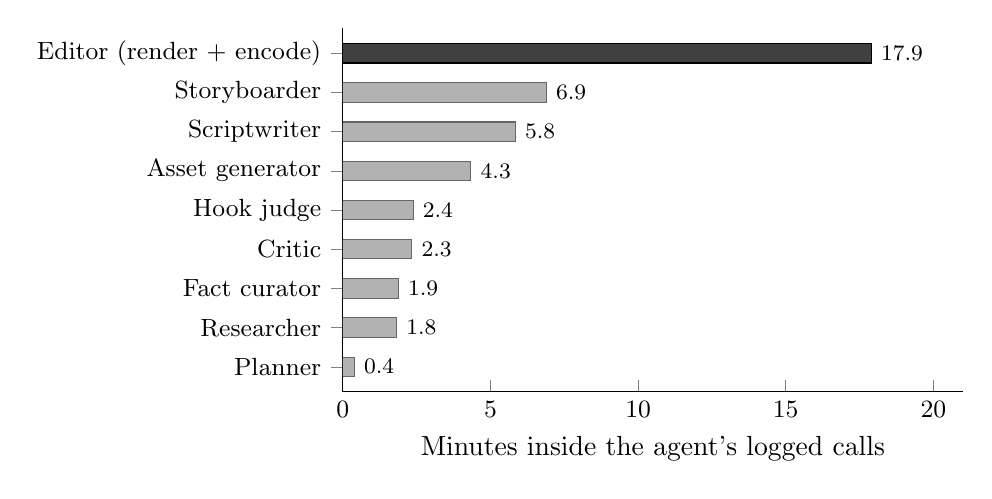
\begin{tikzpicture}
\begin{axis}[
  xbar, bar width=7pt, width=0.78\textwidth, height=6.2cm,
  xmin=0, xmax=21, xlabel={Minutes inside the agent's logged calls},
  ytick={1,...,9},
  yticklabels={Planner, Researcher, Fact curator, Critic, Hook judge, Asset generator, Scriptwriter, Storyboarder, Editor (render + encode)},
  y tick label style={font=\small}, x tick label style={font=\small},
  point meta=x,
  nodes near coords={\pgfmathprintnumber[fixed, precision=1]{\pgfplotspointmeta}},
  nodes near coords style={font=\footnotesize},
  axis x line*=bottom, axis y line*=left, enlarge y limits=0.08,
]
\addplot[fill=black!30, draw=black!60, bar shift=0pt] coordinates
  {(0.39,1) (1.82,2) (1.88,3) (2.34,4) (2.38,5) (4.34,6) (5.84,7) (6.89,8)};
\addplot[fill=black!75, draw=black, bar shift=0pt] coordinates {(17.90,9)};
\end{axis}
\end{tikzpicture}
\caption{Time per agent in the C01 run, summed over the first pass and three repair loops (43.8\,min in total; human review wait excluded). Source: \texttt{logs/run\_log.jsonl}.}
\label{fig:time}
\end{figure}

\paragraph{The repair loop.} The critic found four hard failures in the first pass: the video was 40.3\,s against a 45\,s target, the silent end card counted as dead air, a connective sentence was flagged as an uncited claim, and the end card had no logo. Table~\ref{tab:loops} shows that the scriptwriter fixed the uncited sentence in loop~1, but the other failures persisted through every loop. The logo was a configuration gap that no agent could repair, and the end-card silence was a false positive. Why the duration never changed only became clear after the run (Section~\ref{sec:findings}). After three loops the run went to the mandatory review, where it was approved.

\begin{table}[t]
\centering
\small
\begin{tabularx}{\textwidth}{@{}cr L p{3.2cm}@{}}
\toprule
Pass & Checks & Hard failures & Soft findings \\
\midrule
0 & 51 & duration target, dead air, uncited sentence, end-card logo & caption speed, word budget \\
1 & 55 & duration target, dead air, end-card logo & caption speed, word budget \\
2 & 59 & duration target, dead air, uncited sentence, end-card CTA, end-card logo & caption speed \\
3 & 59 & duration target, dead air, end-card logo & caption speed \\
\bottomrule
\end{tabularx}
\caption{Critic results per pass in the C01 run.}
\label{tab:loops}
\end{table}

\section{Findings From Auditing the Run}
\label{sec:findings}

The reviewer approved the video, and the critic's final report listed only the four failures above. Re-reading the run's artifacts afterwards, and comparing them with frames from the video (Figure~\ref{fig:frames}), showed three defects the critic had not detected.

\begin{figure}[t]
\centering
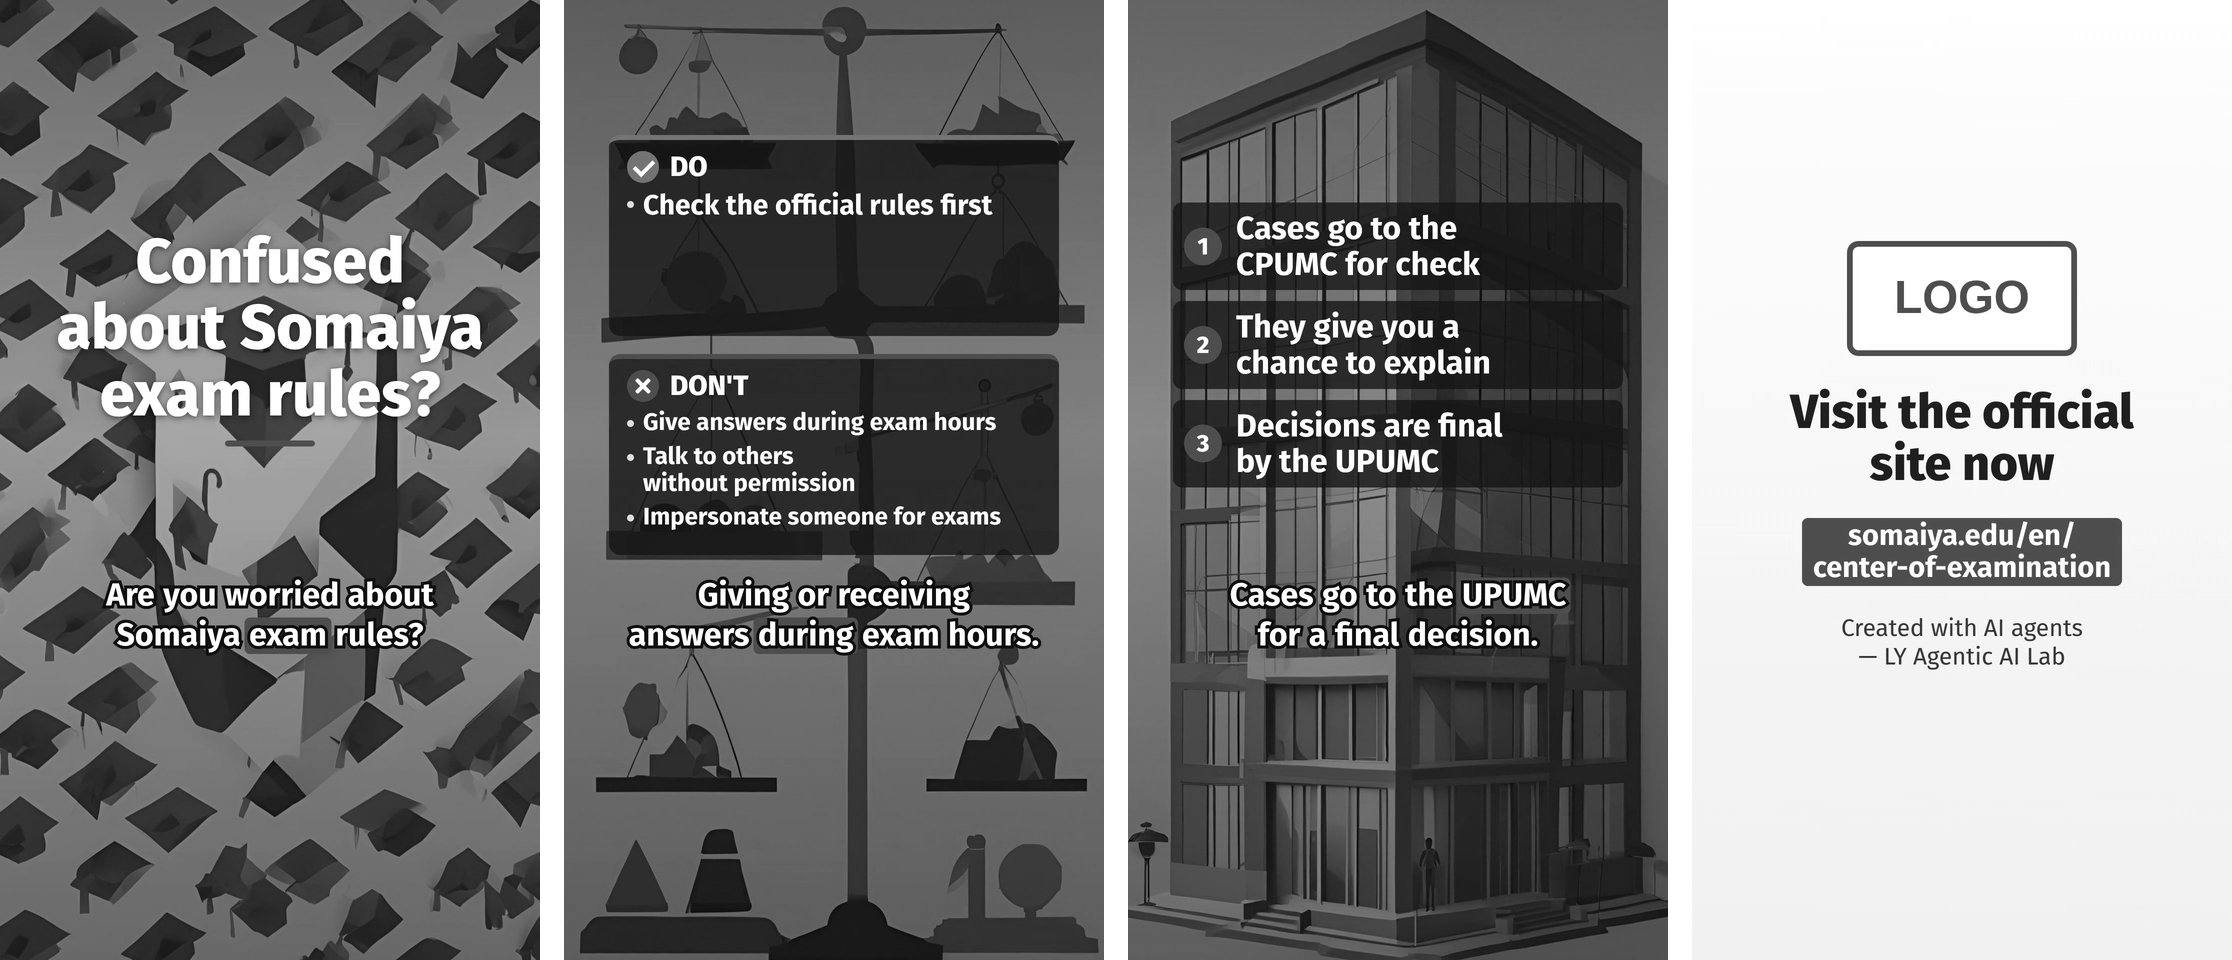
\includegraphics[width=\textwidth]{figures/c01-frames.png}
\caption{Frames from the final C01 render (grayscale). Left to right: hook, allowed-versus-not-allowed card, step list, end card. In the hook the title (``Confused about Somaiya exam rules?'') and the caption (``Are you worried about Somaiya exam rules?'') disagree, and in the step list the cards and the caption describe different steps: the voice-over and captions narrate an earlier script than the one on screen. The building behind the step list is an image generated for an earlier storyboard. The end card shows the placeholder logo.}
\label{fig:frames}
\end{figure}

\paragraph{Stale images.} Images were stored by shot number. When a repair loop re-planned the storyboard, a shot kept the image generated for its predecessor's prompt, so backgrounds stopped matching their shots, and text-only templates inherited images they should not have had.

\paragraph{Stale voice-over and captions.} The voice-over was generated once, in the first pass, and never again. The scriptwriter rewrote the script in every loop, so the critic checked the final script's facts, hook and length while the video narrated the first-pass script, including the sentence the critic had flagged as uncited. The run directory holds a single voice file, and the speech-recognition transcript matches the first-pass script. This is also why the duration never changed: the scriptwriter lengthened the script each loop, but the narration and therefore the video stayed at 35\,s of speech. It also misled our own analysis: we first calibrated the speech rate by pairing the final script's 91 words with the 35\,s voice-over, obtaining 2.6 words per second. The narrated first-pass script has 72 words, so the true rate is 2.1 words per second including pauses, and the earlier calibration would have lengthened the next video by about 10\,s.

\paragraph{Contaminated contact whitelist.} 88 of the 95 whitelisted contacts were URLs from the bibliography of a single government report on AI policy, such as news and journal sites, labelled ``government'' because the document was. A script could have cited any of them as an official link.

\paragraph{Fixes.} Each image now records the prompt it was generated for, and a stale image is regenerated, never reused. The voice-over records a fingerprint of the spoken script it narrates; a stale voice is regenerated before the editor runs, and the critic has a new hard check that the narration is the current script. A URL contact is now judged by its own host and dropped unless the host is official; applied to this run's 95 contacts, the rule keeps 9 (two URLs on official hosts, four e-mail addresses and three phone numbers). The speech rate is set to the measured 2.1 words per second. All fixes have regression tests; the suite now has 120 tests.

\paragraph{Lesson.} All three defects share one cause: a derived artifact (an image, a voice-over, a list of contacts) was trusted without a binding to the exact input it was derived from. The critic checked the right properties on the wrong objects. A check certifies an artifact only if it is bound to that artifact's content, through hashes or fingerprints, and the evidence of the final video itself (OCR, speech recognition) must be compared with what was checked.

\section{Limitations and Future Work}

A fresh Kaggle session spends 25--35\,min downloading models; private Kaggle datasets would remove this. Rendering on four CPU cores is the slowest stage. Generated images can contain small background figures that the face detector does not flag. Government sites with expired certificates or JavaScript-only pages are skipped, and the 30\,MiB fetch cap silently truncates large PDFs such as the UGC regulations; oversized documents should be reported as skipped rather than parsed. The allowlist works at domain level, so pages of sister Somaiya institutions count as official for a KJSCE brief. Contact extraction is literal: it truncated one e-mail address, and it can pick up an individual's e-mail address or mobile number from an official page, which is official but not something a video should publish; today only the human review stands between such a contact and the video. A policy claim can only be grounded in a published document, so C01 cannot describe an AI policy that Somaiya has not published. Finally, the case study is a single run of a single brief; the next steps are a re-run of C01 with the fixes, blind dry runs on Category A and B briefs, and the team's official logo and team identifier in the configuration.

\section{Responsible AI Considerations}

The video discloses that it was created with AI agents. No real person's face or voice is generated: image prompts exclude people for safety and responsible-AI topics, a face detector and a vision model check every frame, and the voice is a stock synthetic voice. Every model and asset is open-licensed and recorded in a manifest. The pipeline never states a policy, statistic or contact that it cannot quote from an official source, and the mandatory human review for Categories A and C puts a person between the pipeline and any safety-critical message.

\acks{We thank Dr Pankaj Mishra, faculty in-charge of the LY Agentic AI Laboratory, and the maintainers of the open-source projects listed in the references, in particular LangGraph, llama.cpp, HyperFrames, Kokoro, faster-whisper and the Qwen models.}

\bibliography{agentreel}

\end{document}
